% ==================================================================
\section{附件2—4的数据核查与预处理}\label{sec:data}
% ==================================================================

从这一章起转入问题二、三。与问题一自己提取特征不同，这两问直接使用附件2—4提供的现成特征。这一章的工作看起来是准备性质的，但后来证明是整个建模过程里最关键的一步：两个问题的技术路线，都是被这里的发现改写的。

\subsection{三个附件的概况}

表\ref{tab:attach}汇总了三个附件的内容。附件2是唯一带标签的数据，模型只能在它上面训练和选型；附件3只有 BERT 的三路整数输入（词元编号、注意力掩码、分段编号），没有现成的文本特征；附件4的20条样本中有5条能按编号在附件2里精确找回，可以当作一个很小的带标签检验集。

\begin{table}[htbp]
\centering
\caption{附件2—附件4概况}
\label{tab:attach}
\begin{tabularx}{\textwidth}{cXcc}
\toprule
附件 & 内容 & 规模 & 标签 \\
\midrule
附件2 & aligned\_50.pkl：text $(50,768)$、audio $(50,74)$、vision $(50,35)$ & 4850 条 & 极性三分类 + 强度 \\
附件3 & text\_bert $(3,50)$、audio、vision & 30 条 & 无 \\
附件4 & 三模态特征 + 原始 mp4 视频 & 20 条 & 无（5条可从附件2找回） \\
\bottomrule
\end{tabularx}
\end{table}

本文采用对齐版特征 aligned\_50.pkl，训练、验证和两个专项测试集全程使用同一版本和同一输入接口。训练集共3395条样本。

\subsection{零帧结构：题目说的缺失，附件2里几乎没有}\label{sec:zero}

我们把每一帧的特征向量求 $L_2$ 范数，小于 $10^{-8}$ 的记为“全零帧”，再按零帧所在位置把它们分成四类：整条全零、尾部连续零段、起始零段、句中零段。图\ref{fig:zeromap}(a)把训练集3395条样本逐行画出来（按语音有效长度排序，深色为零帧），(b)是有效长度的累积分布。

\begin{figure}[htbp]
\centering
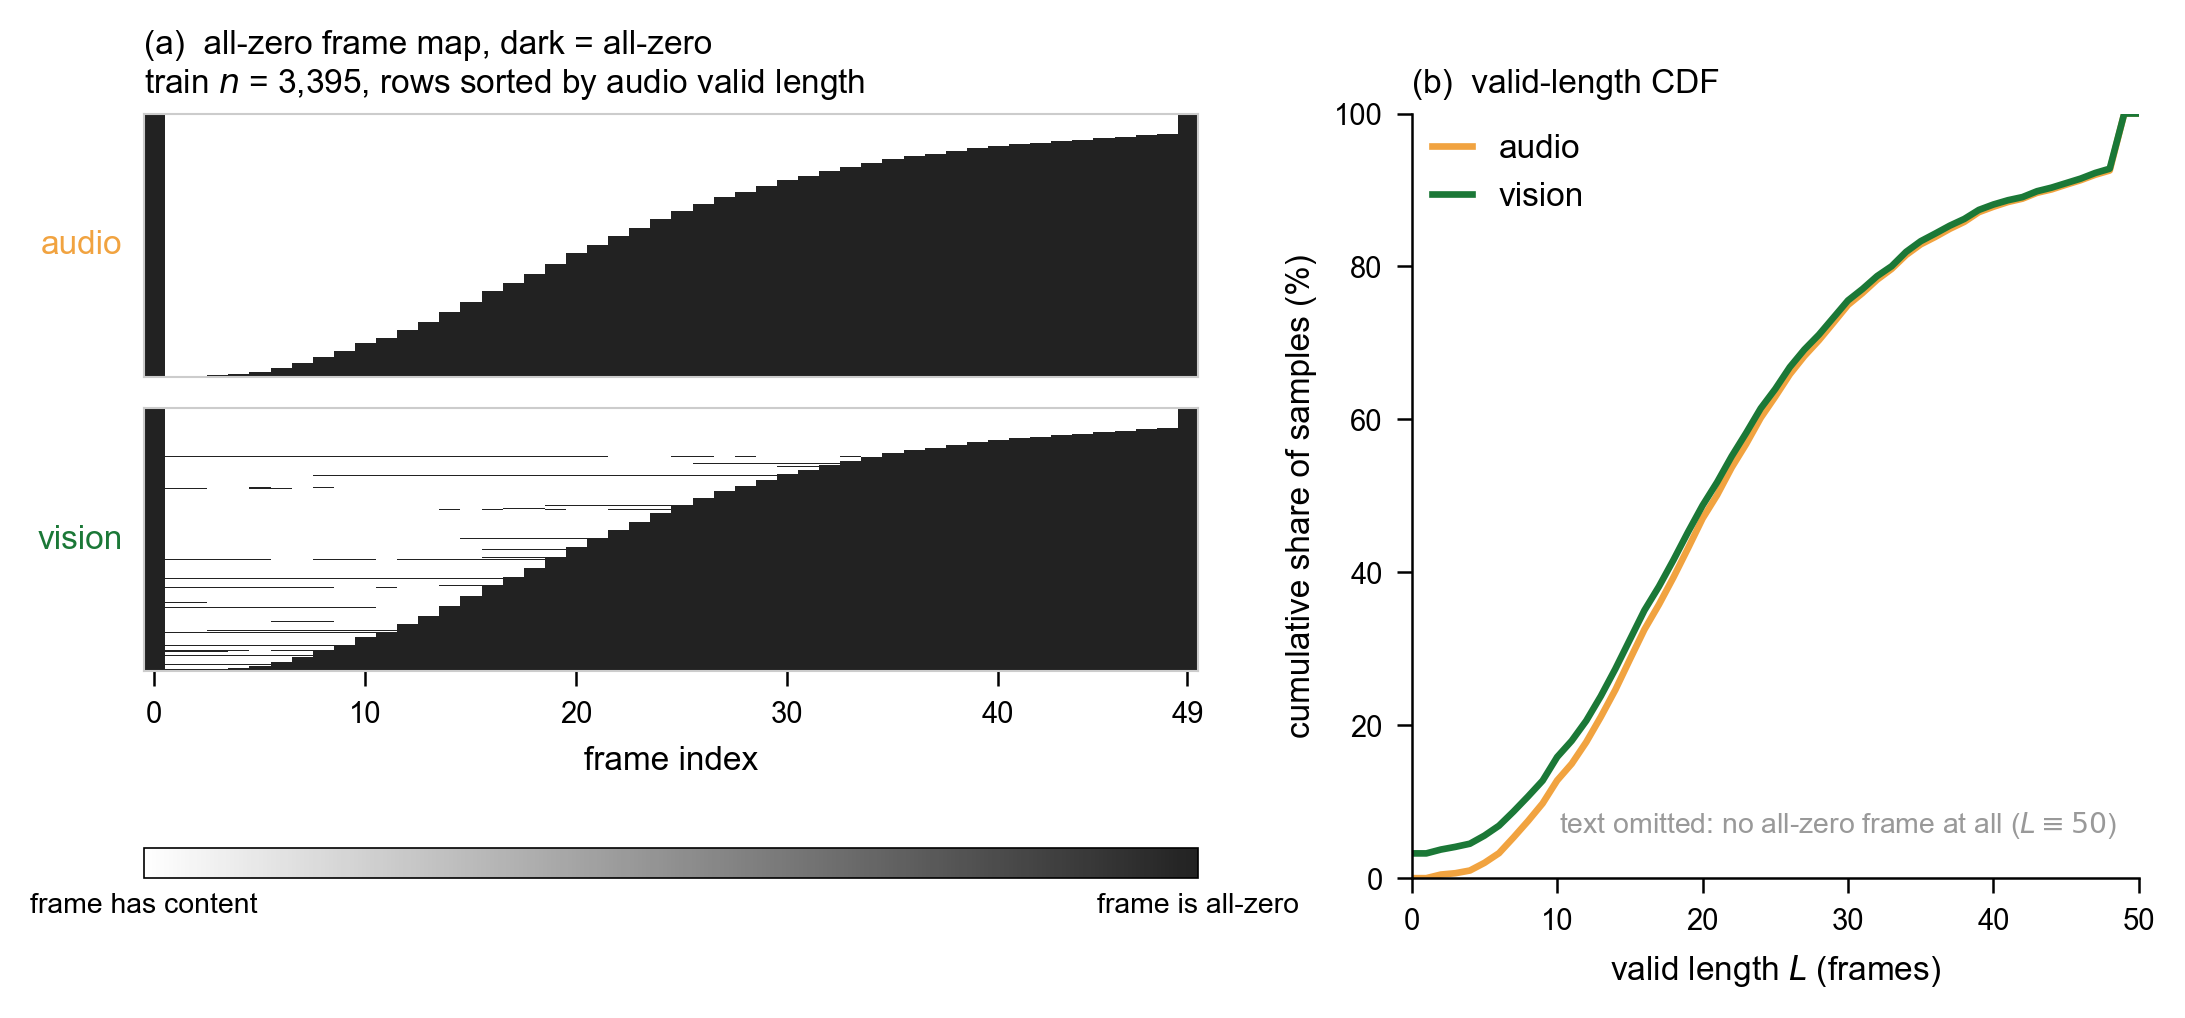
\includegraphics[width=\textwidth]{figures/fig_data_structure.png}
\caption{附件2训练集的零帧分布（a）与有效长度累积分布（b）}
\label{fig:zeromap}
\end{figure}

语音和视觉两张图的阶梯右边界几乎重合，说明两者共用同一段时间轴；文本一行深色都没有，所以没有画出来。有效长度的中位数只有21帧，也就是说一半以上的样本，后面二十多帧全是补齐用的零。表\ref{tab:zero}给出了具体统计。

\begin{table}[htbp]
\centering
\caption{附件2训练集（$N=3395$）零帧统计}
\label{tab:zero}
\begin{tabularx}{\textwidth}{lXl}
\toprule
现象 & 统计结果 & 性质 \\
\midrule
尾部连续零段 & 占零帧比例：语音 96.28\%，视觉 89.18\%；中位长度约29帧 & 变长序列补齐 \\
第0帧全零 & 语音 100\% 的样本，视觉 94\% 的样本 & 对齐产物 \\
句中连续零段 & 语音 0 段，文本 0 段；视觉 210 段（146条，4.3\%） & 零星 \\
文本零帧比例 & 0.0\%（50帧全部有值） & 无缺失 \\
\bottomrule
\end{tabularx}
\end{table}

结论很直接：题目定义的“部分连续时间段不可用”，在附件2的语音和文本上一段都不存在，视觉上也只有4.3\%的样本零星出现。附件2里所谓的连续零段，绝大多数是“这句话本来就这么长”留下的填充。附件3恰好相反，30条样本全部含句中连续缺失（语音30/30，视觉30/30），显然是人为构造的专项测试集。

这个发现改变了问题二的技术路线。如果照搬文献中的缺失设定去训练（整条模态丢弃，或者逐帧独立随机丢弃），模型面对的失效模式和附件3根本不是一回事，训练出来的“鲁棒性”是假的。图\ref{fig:missmodes}把几种形态放在一起对比：(a)是附件2的真实结构，(b)(c)是基线代码中的两种缺失模拟方式，(d)才是题目要求的连续段缺失。四种形态的总体缺失率在42.6\%到58.2\%之间，相差不大，但(b)(c)根本造不出句中的连续段。

\begin{figure}[htbp]
\centering
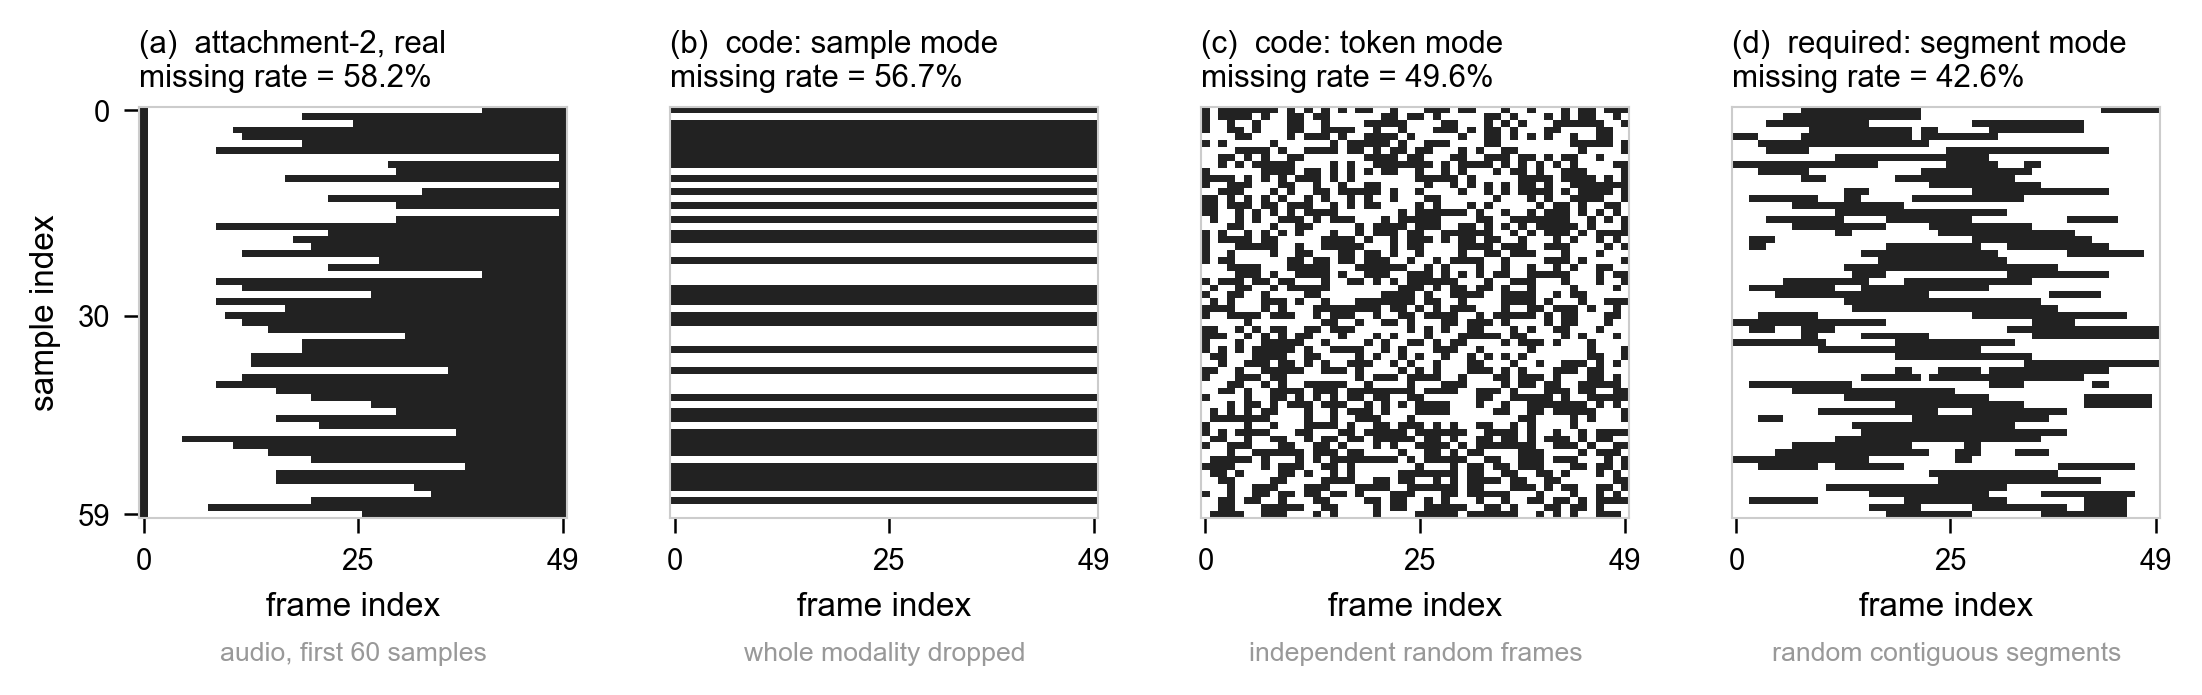
\includegraphics[width=\textwidth]{figures/fig_missing_modes.png}
\caption{缺失形态对比：(a) 附件2真实结构；(b) 整模态丢弃；(c) 逐帧独立丢弃；(d) 连续段缺失}
\label{fig:missmodes}
\end{figure}

\subsection{50个序列位置到底是什么}\label{sec:align}

问题三要求证据“能对应至原始文本片段、语音时段或视觉关键帧”，这逼着我们先弄清楚50个序列位置的物理含义。如果不知道一帧代表什么，所谓的“关键帧”就无从谈起。

如果50帧是按时间等间隔采样的，有效长度应该和片段时长相关。实测结果却是：语音有效长度与文本词元数完全线性相关，
\begin{equation}\label{eq:align}
L_a=\mathrm{nnz}(\texttt{input\_ids})-1,\qquad \mathrm{corr}\big(L_a,\ \#\mathrm{tokens}\big)=1.0000,
\end{equation}
其中 $\mathrm{nnz}(\cdot)$ 表示非零元素个数。该关系在训练、验证、测试三个划分上逐条成立，没有例外。结合 $\texttt{input\_ids}=[\,\texttt{[CLS]},w_1,\dots,w_K,\texttt{[SEP]},0,\dots]$ 的结构可知，第 $t$ 帧对应第 $t$ 个词元：第0帧对应 \texttt{[CLS]}（这也解释了为什么第0帧几乎总是全零），第 $1$ 到第 $K$ 帧依次对应句中的词元。所以这50帧不是时间采样，而是词级对齐。这与问题一中口径H的构造（式(\ref{eq:anchorH})）完全一致：第0帧为零，有效长度等于词元数减1，其后全部补零。问题一选择复刻这一口径，依据就在这里。

由此得到两条后面直接用到的结论：
\begin{enumerate}[label=(\arabic*)]
\item 文本证据可以精确回指：帧号 $\to$ 词元 $\to$ \texttt{tokenizer.decode} $\to$ 原文的词，任何一条证据都能当场人工核对。
\item 语音、视觉只能给“词级锚点”：数据里没有逐词时间戳，只能说“说第 $t$ 个词时的那段语音或表情”，给不出绝对秒数。
\end{enumerate}
对于第二条，我们也考虑过用“平均词长 $\times$ 总时长”估一个秒数，但这样得到的数字误差没法控制，恰恰违背了“可复核”的要求，所以最终只给能给准的东西。

\subsection{预处理}\label{sec:prep}

预处理共三步，做法和理由见表\ref{tab:prep}。

\begin{table}[htbp]
\centering
\caption{预处理步骤}
\label{tab:prep}
\begin{tabular}{>{\raggedright\arraybackslash}p{2.1cm}>{\raggedright\arraybackslash}p{5.6cm}>{\raggedright\arraybackslash}p{5.6cm}}
\toprule
步骤 & 做法 & 原因 \\
\midrule
有效长度提取 & 在标准化\textbf{之前}，从原始特征计算 $L_m$，见式(\ref{eq:validlen}) & 标准化后填充位置的零会变成常数向量，边界就检测不出来了 \\
标准化 & 语音、视觉用训练集统计量做 z-score，见式(\ref{eq:zscore})；文本保持 BERT 原值 & 避免信息泄漏；COVAREP\cite{degottex2014covarep} 语音特征原始值可达500，量纲差异很大 \\
文本重建 & 附件3只有词元编号，用 bert-base-uncased\cite{devlin2019bert} 现场编码 & 已验证附件2的 text 字段就是该模型的 last\_hidden\_state \\
\bottomrule
\end{tabular}
\end{table}

有效长度和标准化分别为
\begin{equation}\label{eq:validlen}
L_m=1+\max\big\{\,t:\ \|U_m^0[t]\|_2>10^{-8}\,\big\},
\end{equation}
\begin{equation}\label{eq:zscore}
\tilde U_m[t,k]=\frac{U_m^0[t,k]-\mu_{m,k}}{\sigma_{m,k}},\qquad m\in\{a,v\},
\end{equation}
其中 $\mu_{m,k}$、$\sigma_{m,k}$ 是训练集第 $k$ 维特征的均值和标准差。

表\ref{tab:prep}第一行的顺序问题是我们实际踩过的坑。最初我们先做标准化，再用标准化后的数据去算有效长度，结果零帧率从55\%一下变成了0\%，所有填充帧都“消失”了。原因就是 z-score 把全零向量变成了常数向量 $(0-\mu)/\sigma$，按范数判断就再也找不到它们。

文本重建一步也做了核对：在附件2上，用同一个 bert-base-uncased 模型对 text\_bert 字段重新编码，得到的结果与现成的 text 字段相关系数为1.0000，平均绝对差为0.0000（保留四位小数）。因此附件3重建出的文本特征与训练数据处在同一个空间里。
